\section{Tratamentos farmacológicos à Depressão}

Os antidepressivos foram descobertos de forma acidental. Ao final da década de 1950, percebeu-se que portadores de tuberculose apresentavam melhoras no humor, ao serem tratados com iproniazida. Contudo, estudos posteriores demonstraram não apresentar eficácia no tratamento da tuberculose. A explicação moderna para a ação da iproniazida consiste na inibição da monoaminoxidase(IMAOs), e a posterior degradação dos receptores de noradrenalina e serotonina(5-HT). O emprego dos antidepressivos IMAOs foi reduzido de forma significativa ao longo do tempo, pois os pacientes vinham apresentando crises sérias de hipertensão.  \cite{Schatzberg2015}

O efeito tardio dos fármacos antidepressivos além de ser um grande enigma científico, é também um problema clínico sério. Os pacientes enquanto aguardam a melhora dos sintomas, podem sentir-se frustrados, podendo interromper o tratamento farmacológico. \cite{Kandel}

Embora a remissão sem recidiva ou recorrência seja a meta procurada pelo tratamento antidepressivo, vem ficando cada vez mais difícil demonstrar que os medicamentos, até mesmo os já estabelecidos, atuam melhor do que o placebo em ensaios clínicos. Embora essa aparente controvérsia sobre a eficácia em ensaios clínicos, no contexto de prática clínica percebe-se que os antidepressivos são importantes agentes terapêuticos em inúmeros pacientes. \cite{Stahl}

\begin{figure}[H]
\centering
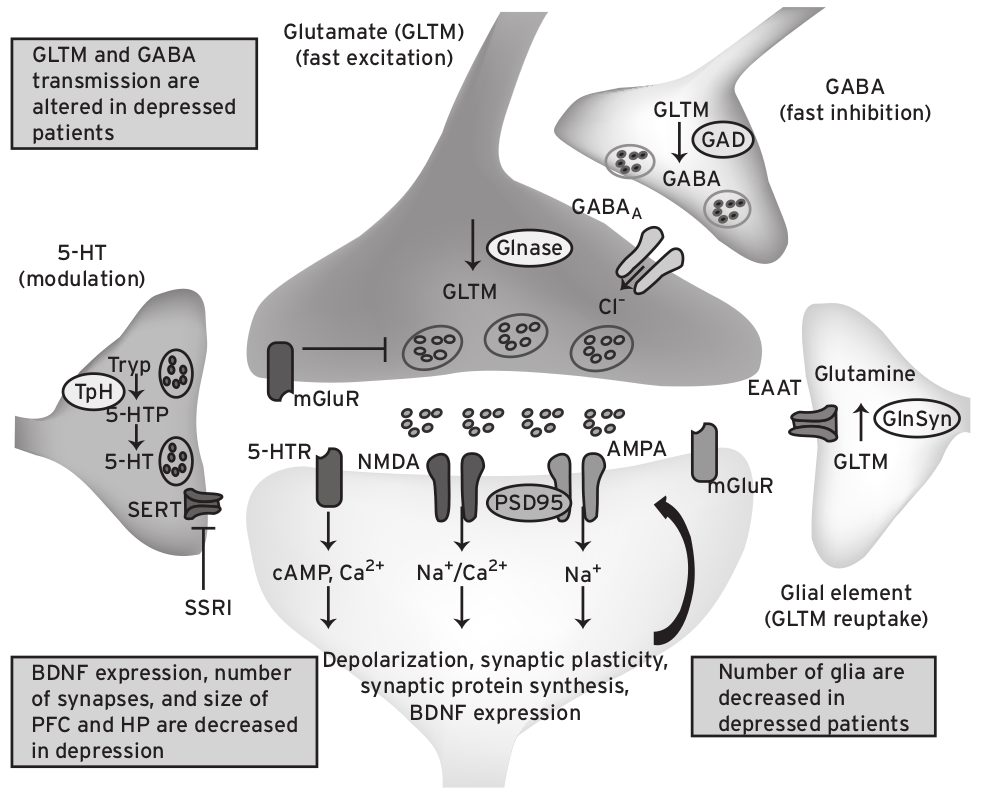
\includegraphics[scale=1.3]{Figuras/glutamate.png}
\caption{Diagrama da transmissão de glutamato e a influência dos neurotransmissores GABA e 5-HT, bem como das células gliais.  \cite{Charney2004}}
\end{figure}

\subsection{A hipótese monoaminérgica}

A ``hipótese monoaminérgica" da depressão, postula que é causada pela diminuição da função da monoamina no sistema nervoso. Os compostos desenvolvidos para condições não psiquiátricas, nomeadamente a iproniazida e a imipramina, tiveram efeitos antidepressivos significativos no ser humano, embora tenham apresentado inúmeros efeitos adversos. Os agentes antidepressivos de hoje oferecem um melhor índice terapêutico e menores taxas de efeitos colaterais para a maioria dos pacientes, mas ainda são projetados para aumentar a transmissão de monoamina de maneira aguda, inibindo recaptação neuronal (por exemplo, inibidores seletivos da recaptação de serotonina (ISRSs), como fluoxetina) ou inibindo a degradação (por exemplo, inibidores da monoamina oxidase, como tranilcipromina). Contudo, a causa da depressão ainda não pode ser explicada mediante uma simples deficiência das monoaminas centrais. \cite{Nestler2008}

A ação clássica dos antidepressivos consiste em bloquear um ou mais dos transportadores de serotonina, noradrenalina e/ou dopamina. Essa ação farmacológica é consistente com a hipótese monoaminérgica da depressão, segundo a qual as monoaminas estão de algum modo deficientes, ocorrendo atenuação dos sintomas depressivos na presença de antidepressivos efetivos. Entretanto, um dos problemas relacionados com a hipótese monoaminérgica é de que a ação dos antidepressivos nos transportadores de monoaminas apesar de elevarem rapidamente os níveis de monoaminas em algumas áreas do cérebro, estranhamente, os efeitos clínicos ocorrem apenas várias semanas depois. \cite{Stahl}

\subsection{A hipótese do eixo hipotálamo–pituitário–adrenal(HPA)}

O estresse é percebido pelo córtex cerebral e transmitido ao hipotálamo, onde o hormônio liberador de corticotropina (CRH) é liberado nos receptores da hipófise(glândula pituitária). Esse estímulo resulta na secreção de corticotrofina no plasma sanguíneo, além de ativar os receptores de corticotrofina no córtex adrenal e liberação de cortisol no sangue. Os receptores de cortisol provenientes do hipotálamo respondem diminuindo a produção de CRH, mantendo a homeostase. \cite{Belmaker2008}

Há importantes evidências de que o cortisol e seu fator central de liberação, o CRH, estão envolvidos na depressão.

\subsection{A hipótese neurogênica}

Evidências crescentes demonstram que a neuroplasticidade, um mecanismo fundamental de adaptação neuronal, é interrompida nos transtornos do humor e perante situações de estresse. O tratamento antidepressivo produz justamente efeitos opostos, podendo aumentar o processo de neurogênese. \cite{Pittenger2008} Diversas pesquisas sugerem que há uma grande correlação entre o sistema neuroimune e os mecanismos de neuroplasticidade sob as condições de depressão. \cite{Eyre2012}

\subsection{Antidepressivos tricíclicos(TCAs)}

Eles são nomeados devido sua estrutura química principal ser composta por três anéis benzênicos unidos. O TCA inicial, imipramina, com estrutura química semelhante às fenotiazinas, foi descoberto na década de 1950 e encontrado por estar associado a melhorias clínicas na depressão. Os primeiros relatos foram feitos pelo professor Kuhn em 1958 na Suíça, onde estudava o tratamento da esquizofrenia e percebeu uma estabilização no humor dos pacientes. \cite{Schatzberg2015}

\subsection{Inibidores Seletivos da Recaptação de Serotonina(SSRIs)}

\begin{figure}[H]
\centering
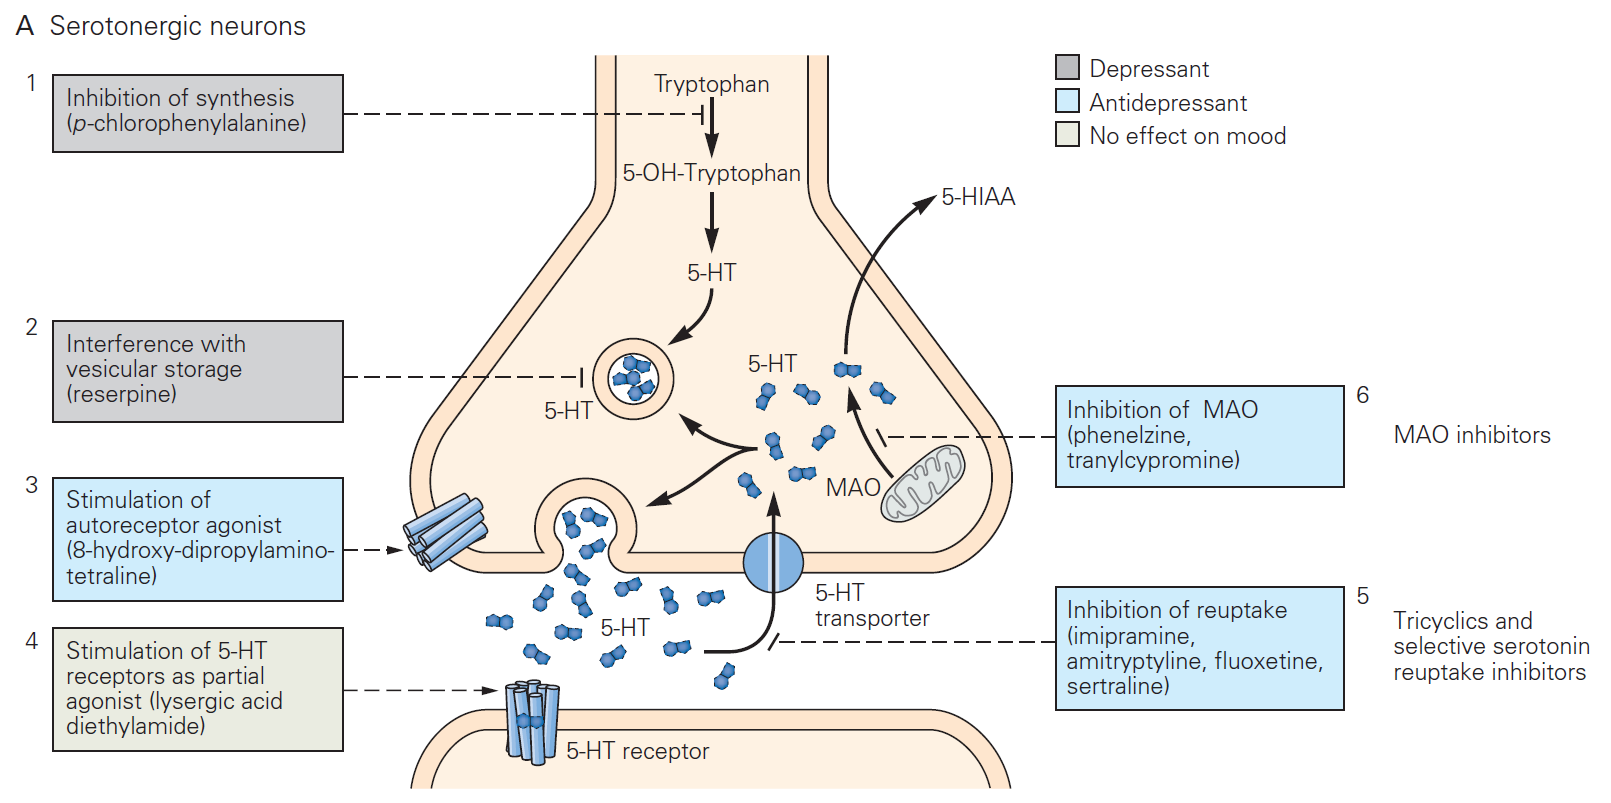
\includegraphics[scale=0.35]{Figuras/serotonergic_neurons.PNG}
\caption{Ação de fármacos antidepressivos nas sinapses serotonérgicas. É apresentado as estruturas pré e pós-sinápticas do circuito de serotonina. \cite{Kandel}}
\end{figure}

O processo de recaptação de serotonina consiste na presença de fármacos antidepressivos, como a fluoxetina ou sertralina, os quais bloqueiam seletivamente os transportadores de serotonina 5-HT. Os fármacos tricíclicos possuem ação mista, onde por exemplo, a clomipramina, são relativamente seletivos. \cite{Kandel} Os ISRSs são a classe mais prescrita de antidepressivos. A versatilidade e sua segurança promovem seu emprego na prática psiquiátrica. Todavia, há relatos desde o início da década de 1990 que os ISRSs propiciam o aumento da tendência suicida, como um dos efeitos adversos. Ainda vem sendo muito difícil discernir um efeito induzido pelo antidepressivo em si, em comparação à progressão da doença subjacente. \cite{Schatzberg2015}

Inicialmente, os ISRSs propiciam um aumento significativo da disponibilidade de serotonina na fenda sináptica. Contudo, os ISRSs também possuem uma ação antidepressiva tardia, semelhante a grande parte dos medicamentos. Percebe-se que conforme a administração recorrente destes fármacos, há uma redução na sensitividade dos receptores $5-HT_{1A}$. Sobretudo, são metabolizados por enzimas hepáticas mediante o citocromo P450. Talvez isto explique, em parte, o certo grau de hepatoxicidade. \cite{Schatzberg2015}

Embora os ADTs tenham sido a classe predominante no mundo por mais de 30 anos, os ISRSs são o de maior popularidade nas últimas décadas. O uso recorrente por parte da prática clínica deve-se em grande parte a sua segurança, e poucos relatos de efeitos adversos graves. Todavia, nem todos os pacientes respondem aos ISRSs, podendo não ter tão eficazes em alguns graus de depressão. \cite{Schatzberg2015} 

\begin{figure}[H]
\centering
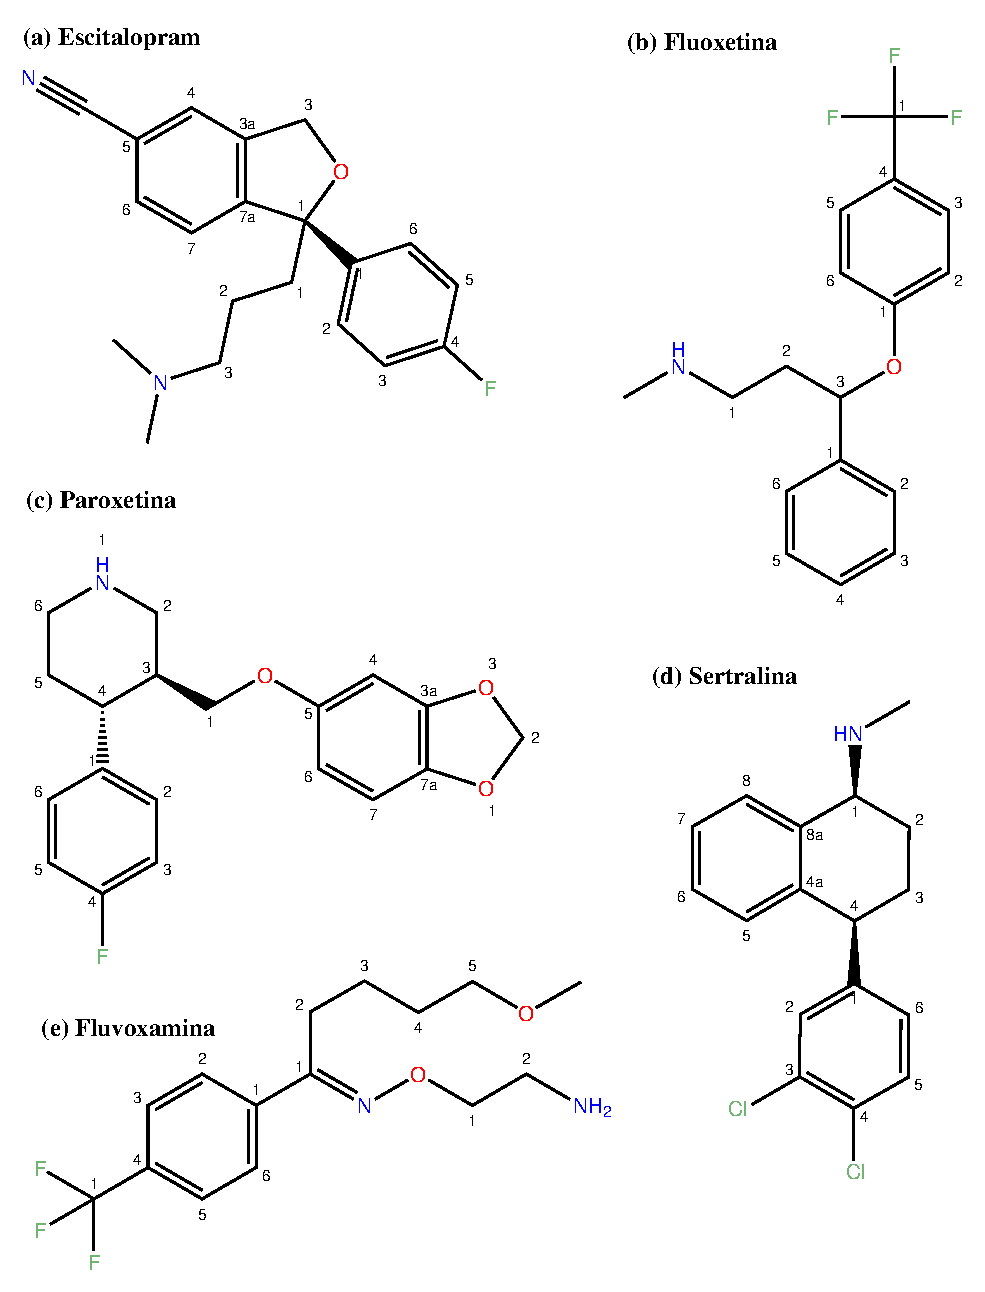
\includegraphics[scale=0.60]{Figuras/isrs.eps}
\caption{Estrutura química dos principais SSRIs comercializados. \cite{Schatzberg2015}} (adaptado)
\end{figure} 

\section{A fronteira da neurociência}

Na próxima década, grande parte dos atuais medicamentos já terão suas patentes expiradas, e darão lugar aos mecanismos mais promissores atualmente. Mediante tudo isso, mostra-se necessário a busca de novos fármacos seguros e eficazes, mas com mecanismos diferentes da antiga hipótese monoaminérgica.  \cite{Nestler2006}

\subsection{A hipótese do sistema de resposta imuno-inflamatório(IRS)}

A teoria das citocinas é certamente a fronteira na ajuda à pacientes com depressão grave. Desta forma, a associação entre inflamação e depressão fornecerá alvos importantes para o desenvolvimento de novos antidepressivos, podendo representar uma esperança a muitas pessoas. Durante vários anos, já vem sido estabelecido que citocinas pró-inflamatórias induzem não apenas sintomas de doenças inflamatórias, mas também estão presentes em transtornos depressivos graves. \cite{Dantzer2008}

\begin{figure}[H]
\centering
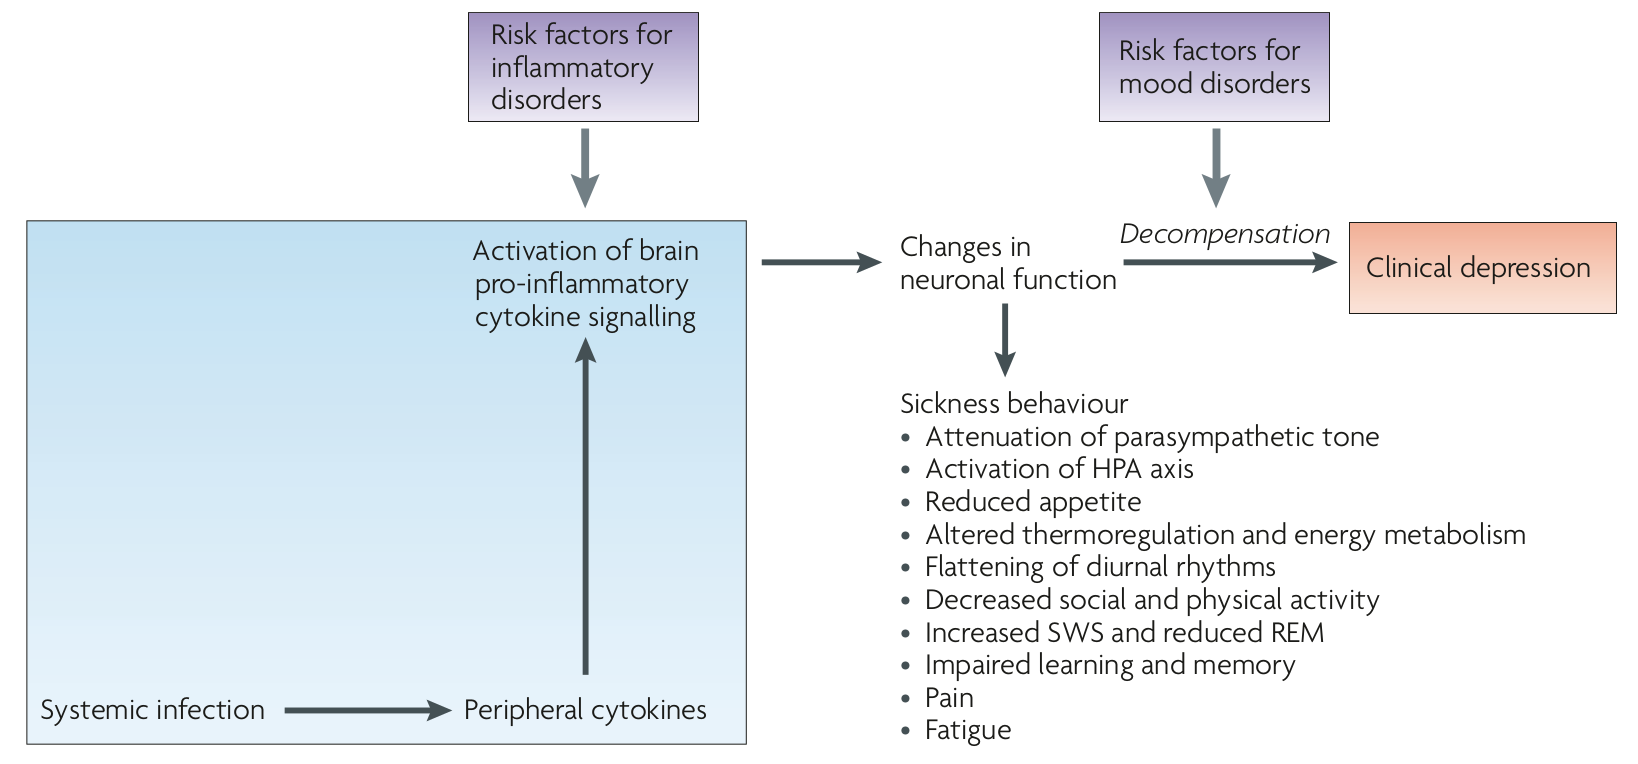
\includegraphics[scale=1]{Figuras/homeostase.png}
\caption{A depressão pode ser vista como consequência de um regime não homeostático de citocinas pro e anti-inflamatórias. \cite{Dantzer2008}}
\end{figure}
